\documentclass[journal]{IEEEtran}

\usepackage{graphicx}

\begin{document}

\title{Reasoning in Artificial Neural Networks}

\author{%
  \IEEEauthorblockN{Vasin Srisupavanich}
}

\maketitle


\begin{abstract}
The abstract goes here.
\end{abstract}


\begin{IEEEkeywords}
Deep learning, neural networks, reasoning, graph neural networks, neural-symbolic, neural turing machine
\end{IEEEkeywords}



\section{Introduction}

\IEEEPARstart{T}{he} ability to reason is one of the most important features of human intelligence. 
It allows us to understand abstract concepts and make complex decisions.
Human excels at tasks that require high level understanding, such as planning and symbol manipulation, 
while the current state of machines are limited to simpler pattern matching problems.
Incorporating reasoning ability to machines has been a long standing goal, but a very difficult challenge in the field of Artificial Intelligence. 
Solving this problem would mean a significant step toward artificial general intelligence, which will ultimately benefits humankind greatly. 
This paper reviews recent approaches in building artificial neural networks that can learn to reason, 
and overview the current state of the art results and applications from deep learning systems with reasoning capability.

\section{Background}
Over the past decade, deep learning systems have enjoyed tremendous success particularly in the area of computer vision and natural language processing.
Machines can now learn to recognize an object in an image with higher accuracy than human, synthesize a novel, and beat a world champion Go player.
However, they still struggle in tasks that involve reasoning operations. For example, deep learning system today have difficulty in
identify cause and effect (causal reasoning), and understanding what is to the left of an object (spatial-temporal reasoning).

Historically, the approach to create an AI system capable of reasoning has been from a symbolic point of view.
In a symbolic AI, knowledge is represented as symbols, rules are handcrafted by human, and reasoning is the process of inference.
However, these systems do not scale to real-world applications, as fixed symbols and rules cannot represents enough information. 
This has paved the way to the current trend of a sub-symbolic deep learning approach, which utilise artificial neural networks. 

With the goal to improve deep learning system beyond pattern matching, AI researchers have tried to combine symbolic AI with neural networks,
which became subfield called Neural-symbolic. Apart from that, researchers also take inspiration from neuroscience. 
As human reasoning involves extracting knowledge from memory and paying attention to specific part of information, 
this has resulted in an extension of neural network in the form of memory and attention mechanism. 

\section{Main Approaches}
\subsection{Attention Mechanism}
Attention mechanism was first introduced in 2014 for a machine translation task \cite{bahdanau2014neural}.
Since then this mechanism has became an important tool for deep learning in various applications. 
This idea is loosely motivated by how human biological system works. For instance, human visual attention allows us to 
focus on specific region with high resolution, while ignoring other irrelevant information. 
In the context of machine translation, attention model enables the machine to focus on specific words at a time 
rather than the full sentence.

In a neural machine translation model (NMT), the architecture consists of an encoder-decoder (seq2seq) structure.
An encoder, typically a recurrent neural networks (RNN), learn to encode a source sentence into a fixed length vector.
Then the decoder network output the encoded vector into another language. Figure \ref{NMT}(a) shows the traditional encoder-decoder architecture.
The apparent problem of this architecture is that the model tends to forget relevant information in a long sentence.
With the addition of attention model (figure \ref{NMT}(b)), this problem is mitigated, 
as the decoder can learn to attend to different parts of the source sentence. 
The attention weights, which are from a feed forward neural networks, are jointly train along with the encoder-decoder networks.

\begin{figure}[htb]
  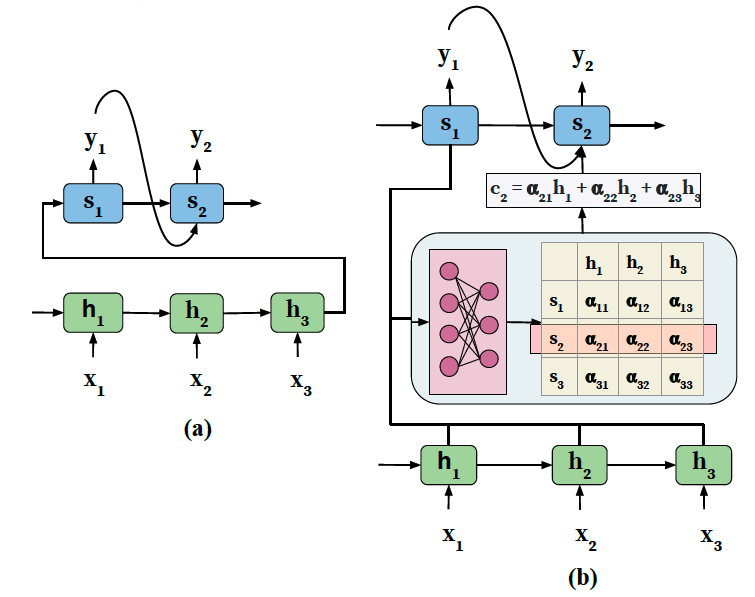
\includegraphics[width=\linewidth]{../NMT.png}
  \caption{NMT architecture (a) traditional (b) with attention model.
  Figure from \cite{chaudhari1904attentive}}
  \label{NMT}
\end{figure}

Another example of how attention 
In \cite{xu2015show}, 
Broadly speaking, there are mainly two types of attention models: soft and hard. 

\subsection{Memory Augmented Neural Networks}

\subsection{Graph Neural Networks}

\subsection{Neural-Symbolic}

\section{Discussion}

\section{Conclusion}

\bibliographystyle{IEEEtran}
\bibliography{references}


\end{document}


